\chapter{Processing - Accumulating the past and future}
\label{ch:preprocess}

\section{Aims}
Representations have a significant affect of what and how quickly a network can learn\cite{akolkar2015can}. 
Thus for any system to predict motion it must necessarily encode some representation of time. 
Traditional approaches to this have been to design Recurrent Neural Networks (RNNs) capable of storing some memory of previous states to inform future decsisions.  
Alternatively a system may make use precise spike timings to encode information as in Spiking Neural Networks (SNNs). 
Many state-of-the-art learning techniques poorly encode time by making the implicit assumption that time is discritised into the frame-rate of the camera used to make a recording.
The decision then seems to be, work with mature state-of-the-art techniques such as deep learning which are poorly able to capture temporal information or RNN/SNNs better suited to process event-based data but with sub--optimal performance.   
However this need not be the case, to leverage the existing literature and use these state-of-the-art models with event-based data, a representation that these networks can accept must be used. 
This section will explore a method of representing event-based data in a frame-based structure while preserving as much temporal information as possible. 


\section{Method}
The simplest solution is to accumulate all the events in a given time slice into a 2D frame to recover images from the event-based data.
This is somewhat counter intuitive though as this forfeits all the temporal information which seperates the DVS from traditional cameras and results in a blury low resolution image. 

\begin{wrapfigure}{r}{0.3\textwidth}
    \centering
    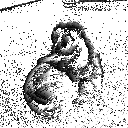
\includegraphics[width=0.3\textwidth]{puppyBall.png}
    \caption{TODO REMOVE THIS IMAGE AND PUT SIMPLE EXAMPLE}
    \label{fig:fadedhistory}
\end{wrapfigure}

An approach to this problem is to choose a distinguished point in time, then construct a 2D image in which each pixels value is a function of its temporal distance to that distinguished point.
If only events that occured prior to the distiguished point in time are considered the resulting image would represent a faded history of what has just happened, this can be seen in figure \ref{fig:fadedhistory} in which a recent history of the scene can be observed. 
Such images can be considered as a faded past, but are also known by many other equivilent names such as; temporal surface, decayed surface, time fields or time surface and these terms can be used interchangeably. 
There is no restriction as to why accumulation can only occur into the past, a similarly interesting image can be produced by accumulating into the future from a distinguished point in time.
These accumulated futures show where objects are moving. 
Consequently if a distinguished point is chosen and an image is accumulated into both the past and future from this point (as per figure \ref{fadedhistory}) these two images can be used as input and labels in a neural netowrk. 


The data is now in a form which can be used in frame-based neural networks and some of the temporal information has been maintained.
Still many questions remain to be explored such as what functions should be used to decay images and with what parameters.


\section{Function specifics and implementation}
%Include a quick maths wise description of this function\\
%Include some resulting images and discussion about each image as to why it is good or bad \\

Two accumulation functions are considered in this work, the first and simplest being linear. 
It can be characterised by equation \ref{eq:linearDecay}, in which the gradient (k) directly affects how much of the past (or future) is considered. 
Here $\Delta t$ is the temporal difference between the closest event for a given pixel and the distinguished point in time. 

% TODO why is this 1/k??

\begin{equation}
 \label{eq:linearDecay}
    f(\Delta t) = 
    \begin{cases}
    -\frac{1}{k}  \Delta t + 1 & 0\leq \Delta t \leq k \\
    0 & Otherwise
   \end{cases}
\end{equation}

An exponential function was also considered as a way to focus on only the most recent history.
Characterised by equation \ref{eq:expDecay} the length of history considered is dependent on the parameter k used. 

\begin{equation}
 \label{eq:expDecay}
    f(\Delta t) = exp\left(\frac{-\Delta t}{k}\right) \\
\end{equation}


%To generate network inputs and outputs distinguished times must be selected and decayed around.
%Each event in the event-stream could be used as a distinguished point and an input/output pair decayed around it.
To generate network input and output images distinguished events must be chosen to be accumulated around.
Every event in the event-stream could be chosen however this would generate a lot of redundant data as many similar events make up any given line.
Rather an event was selected at uniform sequential intervals to be decayed around, that is, every 150th event would be decayed around. 
Additionally after the accumulation into frames the order of training example pairs was randomised and split in 70\% training data, 20\% validation data and 10\% test data. 


\subsection{Parameter influence}
%Show some example parameters and how they affect the data \\
A \textit{k} value seemed problem dependent, interesting values to check first were those corresponding to 1, 16, 33 and 100 (\ms). These values were chosen for similarity to conventional frame-based cameras, 16 and 33\ms corresponding to 60 and 30 frames-per-second cameras respectively. 
The values 1 and 100 \ms were chosen to give some idea of how smaller and larger time scales affected network performance. 
A \textit{k} value is considered to be corresponding to a timeslice when at that temporal distance from the distinguished event the accumulation function gives an output of 0.5.
This is a somewhat arbitrary definition as it may instead make more sense to define a corresponding timeslice to be when the accumulation function gives zero (or near zero). 
As the exponential function will only ever appraoch zero the cut off point will be an arbitrary decision regardless.
In practise using 0.5 was found to perform well as an arbitrary point and meant k values between linear and exponential are comparable.
%TODO include a graphic here demonstrating what corresponding means.
For the linear accumulation function it can be derived that the k values that should be used are given by;

\begin{equation}
    \label{kvalues4linear}
    k = 2 t
\end{equation}

Similarly it can be derived that the \textit{k} values for the exponential case are given by:

\begin{equation}
    \label{kvalues4exp}
    k = \frac{-t}{\ln(0.5)}
\end{equation}

Which when combine result in table \ref{table:kvalues} outlining the choices of \textit{k} to be tested.

\begin{table}[h]
\centering
\begin{tabular}{ | c | c | c | c | c | }
    \hline
    t (\ms) &         1 &     16 &    33 &    100 \\
    Linear &    2 &     32 &    66&     200 \\
    Exp (aprox.)&   1.44 & 23.08 & 47.61 & 144.27 \\
    \hline
\end{tabular}
\caption{Values for k to be test (in milliseconds)}
\label{table:kvalues}
\end{table}

It is worth noting these values are in \ms while the DVS recordings are in \us so the actual \textit{k} values used are 1000 times larger. 


\begin{itemize}
    \item TODO for this section
    \item Decay data as per THOSE k values
    \item Include graphics and comments about those k Values here
    \item Do discussion on them
\end{itemize}

\section{Discussion}

 discuss the selections of k \\
 End up with a blur through time \\
 seems informative to humans at least? \\
 A little bit like a recurrent network (memory of past) \\
 Mention how training, validation and test datasets were generated.\\



